\documentclass{beamer}
\usetheme{Montpellier}
\usecolortheme{beaver}
\usepackage{verbatim}	
\usepackage[square,sort]{natbib}
\usepackage{comment}
\usepackage{amsmath}
\usepackage{caption}
\usepackage{diagbox}
\usepackage{xcolor}
\usepackage{booktabs}

\setbeamerfont{footnote}{size=\tiny}
\setbeamerfont{footnote mark}{size=\tiny}
\setbeamerfont{caption}{size=\scriptsize}
\setbeamerfont{cite}{size=\tiny}

\title{PIRT- Parallel Iterative Reconstruction Tomography, with correction for center of rotation errors}

\author{Sajid Ali\inst{1}, Matthew Otten\inst{2} \& Wendy Di\inst{3}}	
\institute[NU] 
{	\inst{1}%
	Applied Physics\\
	Northwestern University\\
	\inst{2}%	
	HRL Laboratories \\
	\inst{3}%	
	Math. \& Comp. Sci. Divison\\
	Argonne National Lab}

\date{International HPC Summer School 2021 July 2021}

% Delete this, if you do not want the table of contents to pop up at
% the beginning of each subsection:
\AtBeginSubsection[]
{
	\begin{frame}<beamer>{Outline}
		\tableofcontents[currentsection,currentsubsection]
	\end{frame}
}
\AtBeginSection[]{
	\begin{frame}
		\vfill
		\centering
		\begin{beamercolorbox}[sep=8pt,center,shadow=true,rounded=true]{title}
			\usebeamerfont{title}\insertsectionhead\par%
		\end{beamercolorbox}
		\vfill
	\end{frame}
}


\begin{document}

\begin{frame}
\titlepage
\end{frame}

\begin{frame}{Outline}
	\tableofcontents
	% You might wish to add the option [pausesections]
\end{frame}


\subsection{Tomography}
\begin{frame}{Basics}
	\begin{block}{}
		\begin{itemize}
			\item Radon transform : Real $\rightleftarrows$ Sinogram space.
			\item $Rf(\tau,\theta) = 
			\int_{-\infty}^{\infty}\int_{-\infty}^{\infty}
			f(x,y)\delta(\tau - x cos(\theta) - y sin(\theta))dxdy $
		\end{itemize}
	\end{block}
	\begin{center}
		\begin{figure}
			\includegraphics[scale=0.335]{figures/ppa_combined.png}
			\caption{Spinning the object to obatin "sinograms", reconstruct each slice independently. Figure taken from \cite{jacobsen_2019}}
		\end{figure}
	\end{center}
	
\end{frame}

\begin{frame}{Center of rotation drifts}
	\begin{columns}[onlytextwidth,T]
		\column{\dimexpr\linewidth-45mm}
		\begin{block}{}
			\begin{itemize}
				\item $P_{\theta} = x_{\theta}^{*}(1-cos(\theta) + y_{\theta}^{*}sin(\theta))$ 
				\item $Rf(\tau,\theta,0,0) = Rf(\tau - P_{\theta},\theta,x_{\theta}^{*},y_{\theta}^{*})$
				\item Translation of sinogram by $P_{\theta}$ achieved by convolution with Gaussian.
				\item Recover $P_{\theta}$ to obtain accurate reconstruction\footnotemark.
			\end{itemize}					
		\end{block}
		\column{40mm}
		\begin{figure}
			\includegraphics[width=45mm]{figures/drifts.png}
			\caption{Center of rotation drift causes us to measure the shifted sinograms, figure from \cite{wendy_2019}}
		\end{figure}
	\end{columns}
    \footnotetext{\cite{wendy_2019}}
\end{frame}

\begin{frame}{Tomography software}
	\begin{itemize}
		\item Efficient distributed memory parallel tomography software available for CPU and GPU \footnote{\cite{marchesini_inproc_2020, hidayetouglu_inproc_2019, peng_inproc_2019, palenstijn_asci_2016, bicer_asci_2017}}
		\item Error correcting capabilities available in popular tomography packages like TomoPy \footnote{\cite{gursoy_2017}}
		\item Need a software package that has error correction capabilities and is distributed memory parallel
	\end{itemize}
\end{frame}

\subsection{Algorithm \& Implementation}
\begin{frame}{Optimization formulation}
	\begin{block}{Discretize \& Vectorize}
		\begin{itemize}
			\item $\mathcal{W}$ : object vector
			\item $\mathcal{L}$ : discretized Radon transform
			\item $\mathcal{D}$ : measured sinogram
		\end{itemize}
	\end{block}
	\begin{exampleblock}{Least squares cost function}
		\begin{itemize}
			\item Assuming no shifts, we need
			$\underset{\mathcal{W} \geq 0}{\textit{min}}  \frac{1}{2}||\mathcal{L}\mathcal{W}-\mathcal{D}||$
			\item To recover both shifts and object : 
			$\underset{\mathcal{W} \geq 0, P_{\theta}}{\textit{min}}  \phi(\mathcal{W},P_{\theta}) = \frac{1}{2}||\mathcal{L}\mathcal{W} - g(\mathcal{D},P_{\theta})||$
			\item First order derivatives analytically computable :
			$ \nabla \phi(\mathcal{W},P_{\theta}) = [\mathcal{L}^{T},
			\nabla_{P_{\theta}} \phi(\mathcal{W},P_{\theta})]^{T} (\mathcal{L}\mathcal{W} - g(\mathcal{D},P_{\theta}))$
		\end{itemize}
	\end{exampleblock}\end{frame}

\begin{frame}{Implementation}
	\begin{block}{}
		\begin{itemize}
			\item Implemented in C++ using :
			\begin{itemize}
				\item[$\blacksquare$] PETSc/TAO (optimization routines, data management and parallel I/O)
				\item[$\blacksquare$] Boost (geometry routines) 
				\item[$\blacksquare$] FFTW (fourier space convolution)
			\end{itemize}
		\end{itemize}
	\end{block}
	\begin{alertblock}{Joint}
		\begin{itemize}
			\item Combine shifts and sample into one vector and optimize for both together
		\end{itemize}
	\end{alertblock}
	\begin{exampleblock}{Alternating}
		\begin{itemize}
			\item Alternate between optimizing with respect to sample and with respect to shifts
		\end{itemize}
	\end{exampleblock}
\end{frame}

\begin{frame}{Demonstration}
	\begin{itemize}
		\item Quality of reconstructed image and corrected sinograms, with and without error correction.
		\begin{center}
			\begin{figure}
			    %\hspace*{-2cm}
			    \includegraphics[scale=0.185]{figures/result_pirt_2d}
				\caption{Demonstration of PIRT solvers : (Left to Right) with no error correction, alternating solver, joint solver. Test object is $1024^2$ with $200$ projections, with 10$\%$ center of rotation drifts and 10 $\%$ added noise.}
			\end{figure}
		\end{center}
	\end{itemize}
\end{frame}

\begin{comment}
\subsection{Initial refactoring - Summer 2020}
\begin{frame}{History \& Context}
	\begin{block}{History}
		\begin{itemize}
			\item The C++ code began life as a 1:1 port of Matlab code
			\item Buggy and inefficient (serial I/O via C++ fstreams)
			\item Lack of error checking or exceptions, making it difficult to debug especially in parallel
		\end{itemize}
	\end{block}
	\begin{exampleblock}{Context}
		\begin{itemize}
			\item 1.5 years of experience with PETSc from my research on x-ray diffraction algorithms
			\item Some experience with $spack$ after encountering issues with Python package incompatibilities
			\item Some understanding of tomography algorithms
		\end{itemize}
	\end{exampleblock}
\end{frame}

\begin{frame}{Software cleanup \& enhancements}
	\begin{itemize}
     	\item Add error checking from all PETSc routines and fix various bugs
    	\item Cleanup build system by adopting PETSc application makefile, spack environments
    	\item Add basic CI on ANL's internal gitlab instance with some test cases$^{*}$
    	\item Convert all serial I/O to MPI I/O via PETSc's HDF5 interfaces, refactor parallel data structures to reduce communication bottlenecks
    	\item (Stylistic change) Removed multiple classes to have two C++ structs, one for PETSc data, one for Boost data/routines
    \end{itemize}
\end{frame}
\end{comment}

\begin{frame}{Initial Results}
	\begin{center}
		\begin{figure}
			\hspace*{-2.25cm}\includegraphics[scale=0.3125]{figures/drifts_mag_tie}
			\caption{Quality of reconstruction as a function of center of rotation drifts and added noise for an object with dimensions $1024^2$ and $200$ projections, metric $\rightarrow$ translation invariant normalized root mean square error, no regularization.}
		\end{figure}
	\end{center}
\end{frame}

\begin{frame}{Data decomposition}
	\begin{center}
		\begin{figure}
			\hspace*{-1cm}\includegraphics[scale=0.3125]{figures/2d_dist_cropped}
			\caption{Naive data distribution over MPI ranks using PETSc heuristics, with the only constraint being that we don't distribute a single projection over multiple MPI ranks. $ntheta$ $\rightarrow$ number of projections, $ntau$ $\rightarrow$ size of each projection.}
		\end{figure}
	\end{center}
\end{frame}

\begin{frame}{2D solve scaling}
	\begin{itemize}
		\item Tests conducted on LCRC-bebop, dual-socket Xeon Broadwell, Intel Omni Patch interconnect.
	\end{itemize}
	\begin{columns}[onlytextwidth,T]
		\column{\dimexpr\linewidth-45mm}
		\begin{figure}
			\hspace*{-1cm}\includegraphics[scale=0.4]{figures/strong_scaling}
			\caption{Strong scaling $\rightarrow$ object size $2896^2$,\\ $800$ projections. }
		\end{figure}
		\column{40mm}
		\begin{figure}
			\hspace*{-1cm}\includegraphics[scale=0.4]{figures/weak_scaling}
			\caption{Weak scaling object size $\rightarrow$ $1024^2$, projections per node $100$}
		\end{figure}
	\end{columns}
\end{frame}

\subsection{3D solver}
\begin{frame}{Research choices}
	\begin{itemize}
		\item Profiling showed some improvement post enhancements but strong and weak scaling efficieny falls off beyond 4 nodes for a single 2D slice solve. 
		\item Reason being the naive data distribution leading to load balancing issues, $\approx80$ of time being spent in matrix-vector and transposed matrix-vector multiplications. 
		\item However, experimental data is always a 3D data-set! Focus on throughput instead of scalability of a single 2D slice solve. 
		\item Introduced MPI-subcommunicator based 2-level MPI parallelism, with multiple concurrent instances of the solver.
	\end{itemize}
\end{frame}

\begin{frame}{2 level MPI parallelism}
	\begin{center}
		\begin{figure}
			\hspace*{-1cm}\includegraphics[scale=0.3125]{figures/2level.png}
			\caption{(Left) Architecture of the 2-level parallelism. Each solver instance solves for a "batch" of 2D slices (Right) Idea on accelerating convergence of 3D solver by combining results of 2D solves. To combine the shifts from subcomms, run multiple "overall sweeps" with checkpoint-restart. }
		\end{figure}
	\end{center}
\end{frame}

%\begin{frame}{Effect of sweeps}
%	\begin{itemize}
%		\item Odd behavior of TAO solvers for iterations $>$ 1 : accumulated QN Hessian approximation is not reset for each new TaoSolve %call!
%		\item Observed that the joint solver benefits from multiple restarts ("sweeps") from checkpointed sinogram even for one slice.
%		\item No clear benefit from combining shifts across concurrent solvers, but some benefit from re-using shifts within each batch. %However, this benefit is rather fragile to obtain in practice and no mathematical basis for it.
%	\end{itemize}
%\end{frame}

\begin{frame}{Throughput Results}
	\begin{center}
		\begin{figure}
			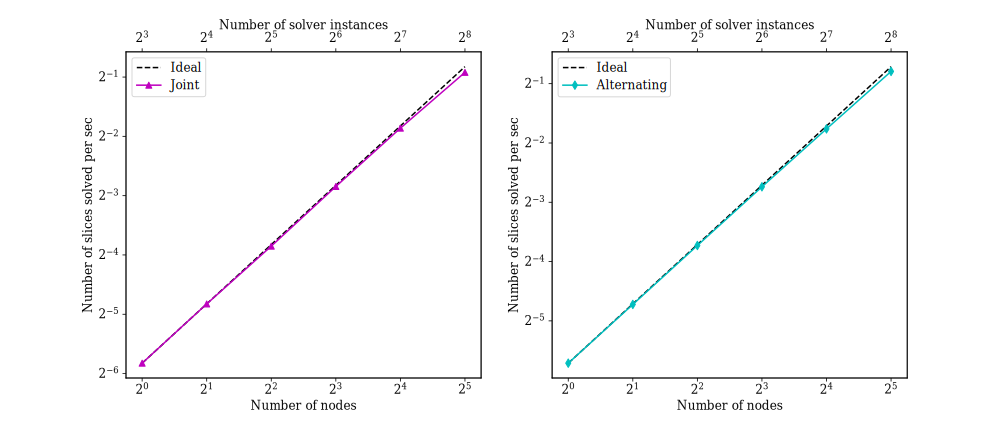
\includegraphics[scale=0.3125]{figures/throughput}
			\caption{Number of slices solved per unit time, 256 slices of size $1024^2$ and $200$ projection angles. Tests conducted on LCRC-bebop, dual-socket Xeon Broadwell, Intel Omni Patch interconnect.}
		\end{figure}
	\end{center}
\end{frame}

\begin{comment}
\subsection{GPU Port}
\begin{frame}{Pre-hackathon port path \& Goals }
	\begin{block}{GPU Port path : }
		\begin{itemize}
			\item FFTW $\rightarrow$ cuFFT 
			\item CUB for block-wise reductions
			\item remaining $for$ loops $\rightarrow$ CUDA kernels
		\end{itemize}
	\end{block}
    \begin{exampleblock}{Goals}
	  \begin{itemize}
		\item Focus on porting the TAO objective function $\&$ gradient routines in addition to some helper routines
		\item Profile GPU versions to ensure that the port is efficient
		\item If the single slice, single instance solver works, begin investigation of running concurrent solver instances
      \end{itemize}
    \end{exampleblock}
\end{frame}

\begin{frame}{Change in strategy}
  \begin{block}{Surprises!}
	\begin{itemize}
		\item Typically, $>90\%$ of total time is spent in objective function/gradient routines, but on theta-gpu, $<5\%$
		\item Bottleneck : setting up non-contiguous data transfers between GPU arrays for bounds projection from estimated active set
    \end{itemize}
  \end{block}	
  \begin{exampleblock}{Alternatives to explore}
    \begin{itemize}
      \item Remove bound constraints $\rightarrow$ solution quality degrades
      \item Re-evaluate for problem sizes of interest to APS beamlines ?
      \item If the active-set estimation/bound projection bottleneck still exists, explore alternate formulations like Augmented Lagrangian multiplier method
   \end{itemize}
  \end{exampleblock}
\end{frame}

\begin{frame}{Results and Final Profile}
\begin{table}[]
	\centering
	\scalebox{0.85}{
	\begin{tabular}{lllllllll}
		\toprule
		& \multicolumn{2}{l}{1 MPI Rank} & \multicolumn{2}{l}{4 MPI ranks} & \multicolumn{2}{l}{8 MPI Ranks} & \multicolumn{2}{l}{16 MPI Ranks} \\ 
		& Total     & \% f/g    & Total     & \% f/g    & Total     & \% f/g    & Total     & \% f/g     \\ \midrule
		
		\textcolor{cyan}{CPU-joint} & 899.0 & \textcolor{cyan}{89.7} & 250.2 & \textcolor{cyan}{84.1} & 134.4 & \textcolor{cyan}{84.8} & 79.0 & \textcolor{cyan}{86.5}     \\
		
		\textcolor{magenta}{GPU-joint} & 128.8     & \textcolor{magenta}{2.9}  & 66.2      & \textcolor{magenta}{5.8} & 37.8      & \textcolor{magenta}{12.4}      & 58.9      & \textcolor{magenta}{21.3}       \\ \midrule
		
		\textcolor{cyan}{CPU-alt}   & 765.9     & \textcolor{cyan}{97.6}      & 185.8     & \textcolor{cyan}{96.4}      & 100.4     & \textcolor{cyan}{96.5}      & 58.8      & \textcolor{cyan}{96.8}       \\
		
		\textcolor{magenta}{GPU-alt}  & 22.5      & \textcolor{magenta}{12.7}      & 11.8      & \textcolor{magenta}{17.4}      & 9.5       & \textcolor{magenta}{30.0}      & 22.4      & \textcolor{magenta}{54.1}       \\ 
	    \bottomrule
	\end{tabular}
    }
    \caption{\label{tab:table-name}Analysis of total time as a function of MPI ranks for CPU and GPU solves and $\%$ of time spent in evaluation objective function and gradient. Object size $1024^2$, $200$ projection angles.}
\end{table}
\end{frame}
\end{comment}

%\section{Acknowledgments}
\begin{frame}{Acknowledgments}
	\begin{itemize}
		\item \alert{Wendy Di} MCS/APS-ANL, internship \& thesis advisor
		\item \alert{Matthew Otten} CNM-ANL, internship co-advisor
		\item \alert{Chris Jacobsen} NU \& XSD-ANL, thesis advisor
		\item \alert{Alp Dener}, TAO-developer, MCS/ANL
		\item \alert{Hong Zhang/Barry Smith}, GPU hackaton mentors/PETSc developers, MCS/ANL
		\item \alert{PETSc developers} on the mailing lists
		\item \alert{bebop-LCRC} ANL \& \alert{theta-GPU} ALCF for resources
		\item \alert{NIMH} \& \alert{ANL-MCS} for funding
	\end{itemize}
\end{frame}

\renewcommand*{\bibfont}{\scriptsize}
\begin{frame}[t, allowframebreaks]
	\frametitle{References}
	\bibliographystyle{dinat-etal}
	\bibliography{pirt}
\end{frame}

\end{document}
